\section{Data Structures and Mesh Traits}
\label{chap:mesh-traits}

One of the main challenges in creating this library was to find a suitable set of traits that would serve as a reasonable abstraction over different mesh data structures.
A single trait is not sufficient because not all data structures offer the same set of capabilities.
On the other hand, having one trait for each individual feature (i.\,e., for each neighborhood~information, each mutating operation, \dots) would result in a very large number of traits, making the library's API much harder to understand and more difficult to work with.
Finding a good solution in between those extremes is crucial for the usefulness of the abstraction.
This section describes the design considerations and introduces a few possible solutions.

As a first step, it is important to define what entities should be abstracted over.
As mentioned, the main goal is to be able to easily switch between different mesh data structures, which are provided by \code{lox} itself.
But users of this library can also implement the traits for their own types, allowing them to use many features (like mesh algorithms or IO) without \code{lox} even knowing about those data structures.
It can thus be beneficial to imagine what other types could reasonably implement the mesh traits.
This could include basic graph data structures, implicitly defined polygon meshes or other highly specialized data structures.
To reduce the scope of this problem, this thesis focused on known mesh data structures provided by \code{lox}.

Finding a good design for such a central interface requires knowledge about everything that interacts with it and a fair amount of experience from working with different solutions.
While quite some experience was gained during \code{lox}'s development so far, it is not sufficient to commit to one specific solution (in the opinion of the author).
Instead, a few more design iterations are to be expected.
In particular, since the library was not yet (as of this writing) publicly released, other programmers did not have the chance to provide feedback.


\subsubsection*{Basic and Optional Capabilities}

A good starting point is to define the basic features of a \enquote{mesh} (the lowest common denominator) and to identify \emph{optional} capabilities.
All basic features are defined in the trait \code{Mesh} (in OOP\footnote{Object Oriented Programming} terms: the very top of the class hierarchy).
Describing the optional capabilities (i.\,e., the features not part of \code{Mesh}) in the trait system is the main challenge in finding a good design.
Note that for now, adjacency information is ignored.

Different data structures can expose different elements in their API: faces, vertices, edges and half-edges.
Elements that are not exposed cannot be referred to and thus, associating data with those elements is not possible.
For exposed elements, we expect the data structure to be able to enumerate all elements of that kind (i.\,e., iterate over them).
As faces and vertices are needed in almost all situation and since they can be exposed by all data structures discussed so far, they are considered a basic part of meshes and are included in \code{Mesh}.
However, edges are not exposed by all data structures and are thus optional, referred to as \code{EdgeMesh} from here on.
Exposing half-edges can be useful in many situations, but they are not as important as full edges.
Therefore, as well as to reduce the scope during initial development, half-edges were ignored for the public API (of course, half-edges can still be used internally by data structures).

Another optional capability is \emph{mutability}.
Not all algorithms need to modify meshes and it is conceivable that some more exotic data structures (e.\,g., implicitly defining the mesh) do not support mutation.
As such, it makes sense to treat the ability to mutate the mesh as an optional capability, called \code{MeshMut}.

The distinction between pure triangle meshes and polygon meshes also needs to be considered.
While it makes intuitive sense that polygon meshes offer an additional feature by letting algorithms create non-triangular faces, pure triangle meshes also offer additional features as some operations are only possible on triangle meshes.
So these are two mutually exclusive, optional capabilities with the extra restriction that each mesh should offer exactly one of them.
They are referred to as \code{TriMesh} and \code{PolyMesh} from here on.
(In the future, pure quad meshes will be considered in the API, too.)

Everything a mesh data structure has to offer now belongs to one of three categories (see figure~\ref{fig:mesh-features} for an overview):

\begin{itemize}
  \item \textbf{Basic mesh features}. For example: enumerating all vertices.
  \item \textbf{Requires \emph{one} additional capability}. For example: \code{add_vertex} (requires mutability) or enumerating all edges (requires exposed edges).
  \item \textbf{Requires \emph{multiple} additional capabilities}. For example: \code{add_face} (add face with arbitrary valence, requires mutability and \code{PolyMesh}) or \code{flip_edge} (requires mutability, \code{EdgeMesh} and \code{TriMesh}). % TODO: add figure showing edge flip
\end{itemize}

\begin{figure}[t]
  \centering
  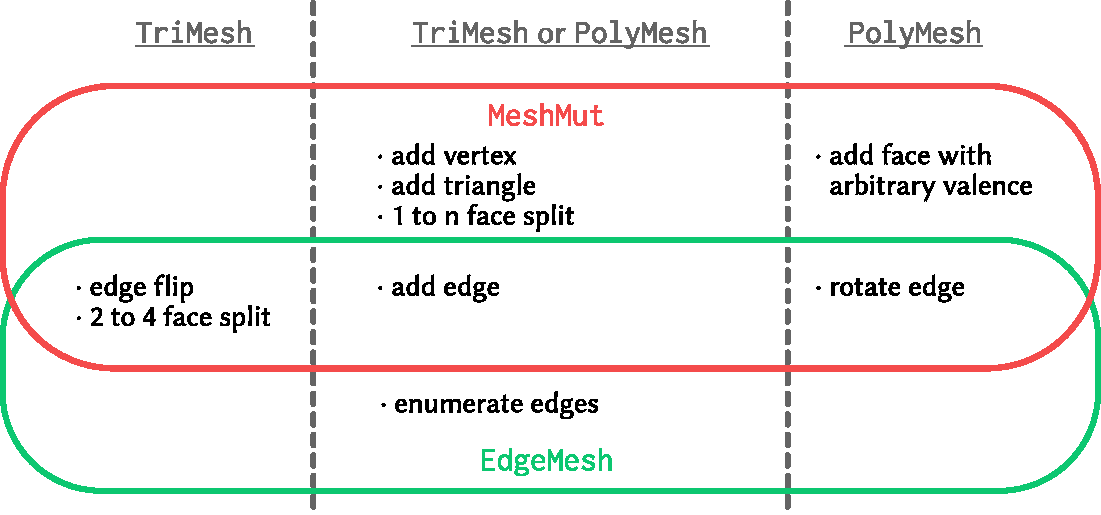
\includegraphics[width=.98\textwidth]{svg2pdf/mesh-features}
  \caption{
    A couple of example mesh features categorized by which capabilities they require (this diagram is not complete).
  }
  \label{fig:mesh-features}
\end{figure}

As already stated, basic mesh features are defined in \code{Mesh}.
There are multiple possibilities where all other features are defined:

\begin{itemize}
  \item Create a trait per combination of capabilities (e.\,g., \code{PolyMeshMut} for triangular meshes that can be mutated) and put each feature in the fitting trait.
  This works, but creates a large number of traits.
  Users might prefer to have functionality in as few traits as possible.
  \item Create a trait per single optional capability and put features only requiring one capability in the corresponding trait.
  Features requiring multiple capabilities are defined in the trait of one of those capabilities, defining all other capabilities by adding trait bounds to \code{Self}.
  For example, the method to add arbitrary faces could be defined in \code{MeshMut} with the following signature:

  \begin{rustcode}
    fn add_face(&mut self, vertices: &[VertexHandle]) -> FaceHandle
    where
        Self: PolyMesh;
  \end{rustcode}

  \item Like the last version, but put all methods into \code{Mesh}, completely declaring the required capabilities via bounds on \code{Self}.
  \item Some combination of the three explained possibilities.
\end{itemize}

None of these solutions is clearly better than the others which is part of the reason the design of the mesh traits is not finished yet.
The current solution is to define all methods in either \code{Mesh} or \code{MeshMut}.
Traits \code{EdgeMesh}, \code{TriMesh} and \code{PolyMesh} are added, but just serve as markers.
Methods requiring additional capabilities declare that via bounds on \code{Self}.
This design avoids having a large number of traits and all functionality is found in only two traits, making it easy to discover for users.
Also see figure~\ref{fig:mesh-traits}.

\subsubsection*{Mutually exclusive traits}

Special attention has to be paid to the design of \code{TriMesh} and \code{PolyMesh}.
Simply adding two traits would be incorrect, because types could implement neither or both of these traits which should be prohibited.
To solve this problem, the trait \code{Mesh} could declare an \emph{associated constant} and the two traits could be defined in terms of this constant:

\begin{rustcode}
  enum FaceKind { Triangle, Polygon }

  trait Mesh {
      const FACE_KIND: FaceKind;
  }

  trait TriMesh: Mesh<FACE_KIND = FaceKind::Triangle> {}
  trait PolyMesh: Mesh<FACE_KIND = FaceKind::Polygon> {}

  // Blanket implementation to automatically implement traits for all types
  // that also implement Mesh with the correct face kind.
  impl<T: Mesh<FACE_KIND = FaceKind::Triangle> TriMesh for T {}
  impl<T: Mesh<FACE_KIND = FaceKind::Polygon> PolyMesh for T {}
\end{rustcode}

Implementors need to define a value for the constant when implementing the trait.
\code{TriMesh} and \code{PolyMesh} are automatically implemented for these types implementing \code{Mesh} with the corresponding value.
The only problem with this approach is that it does not compile yet:
the Rust compiler still lacks the ability to check value equality within trait bounds.
Luckily, this problem can simply be worked around by using types instead of values and using an associated type instead of an associated constant.

\begin{rustcode}
  // Two types instead of two values.
  enum TriFace {}
  enum PolyFace {}

  // A trait which is only implemented for these types (not strictly
  // necessary, but avoids misuse of the API).
  trait FaceKind {}
  impl FaceKind for TriFace {}
  impl FaceKind for PolyFace {}

  trait Mesh {
      type FaceKind: FaceKind;  // Type instead of constant
  }

  trait TriMesh: Mesh<FaceKind = TriFace> {}
  trait PolyMesh: Mesh<FaceKind = PolyFace> {}

  // Blanket implementation to automatically implement traits for all types
  // that also implement Mesh with the correct face kind.
  impl<T: Mesh<FaceKind = TriFace> TriMesh for T {}
  impl<T: Mesh<FaceKind = PolyFace> PolyMesh for T {}
\end{rustcode}


\subsubsection*{Adjacency Traits}

All functionality regarding adjacency information has to be defined in traits as well.
As before, defining too many traits (e.\,g., one trait per basic adjacency query) would make the whole API more confusing while a single trait would not be flexible enough.
The current design consists of three traits (cf. figure~\ref{fig:mesh-traits}):

\begin{itemize}
  \item \textbf{\codebox{BasicAdj}}: this trait only defines \adj{F}{V} adjacency.
  This is arguably the most used neighborhood query as it is needed for basic rendering and IO.
  The trait is implemented by all mesh data structures within \code{lox}.
  \item \textbf{\codebox{FullAdj}}: requires \code{BasicAdj} and adds \adj{F}{F}, \adj{V}{F} and \adj{V}{V} queries, meaning that all queries between faces and vertices are supported.
  It is implemented by all data structures except for \code{SharedVertexMesh}.
  \item \textbf{\codebox{EdgeAdj}}: requires \code{FullAdj} and adds \adj{E}{F}, \adj{E}{V}, \adj{F}{E} and \adj{V}{E}.
  This is currently only implemented by \code{HalfEdgeMesh}.
\end{itemize}

This solution works fairly well for mesh data structures defined within \code{lox}, but has not been evaluated for potential external data structures:
The main advantage is the low number of traits which simplifies the API.
But as mentioned above, this design is likely to change in the future.

\begin{figure}[th]
  \centering
  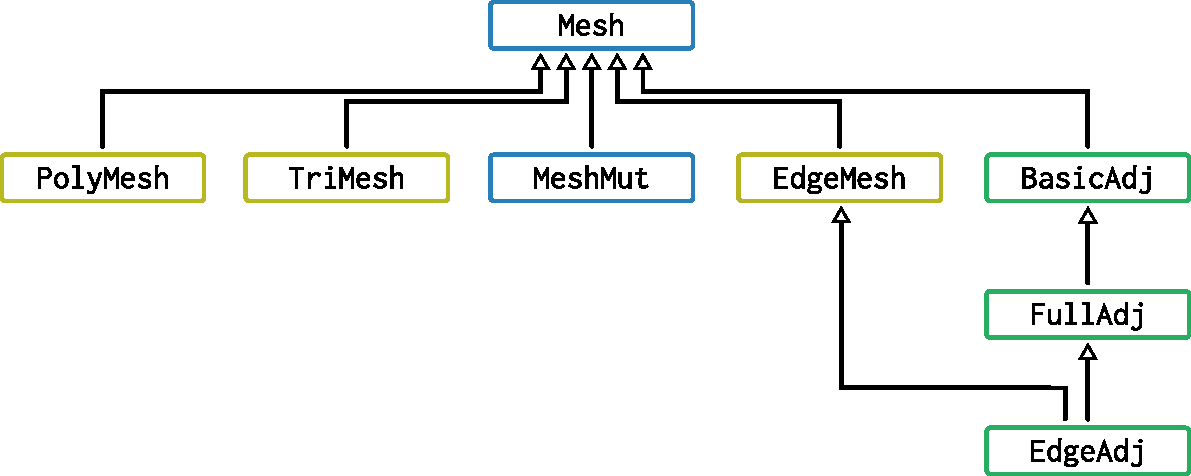
\includegraphics[width=.98\textwidth]{svg2pdf/mesh-traits}
  \caption{
    Traits currently used in \codebox{lox} to abstract over meshes.
    The arrows represent \emph{super trait bounds}, i.\,e., \codebox{Mesh} is a super trait of \codebox{MeshMut}.
    Green boxes contain traits that deal with adjacency information, yellow boxes indicate marker traits without own methods.
  }
  \label{fig:mesh-traits}
\end{figure}


\vfill
\subsubsection*{Data Structures in \codebox{lox}}

At the time of this writing, \code{lox} provides three data structures:
the shared vertex mesh, the half edge mesh and the directed edge mesh.
However, it is planned to add more data structures to the library in the near future.

%TODO: maybe actually implement this?
The half edge mesh and directed edge mesh can be configured at compile time.
Both meshes allow specifying which optional fields (e.\,g., \code{prev}) are stored and the half edge mesh offers an option to restrict the mesh to triangular faces (which does not change the underlying data structure, but makes some operations faster).
The configuration is done via a type parameter and a trait \code{Config}.
The system for the half edge mesh looks like this:

\begin{rustcode}
trait Config {
    type FaceKind: FaceKind;
    type StorePrev: Bool;
}

struct HalfEdgeMesh<C: Config> { /* ... */ }

// Type-level bool
trait Bool {}
enum True {}
enum False {}
impl Bool for True {}
impl Bool for False {}
\end{rustcode}

As mentioned previously, Rust does not yet support using constants in trait bounds.
For that reason, the \code{Config} trait uses associated types instead of associated constants to store type-level values.
The \emph{FaceKind} trait is the one defined earlier in this section.

\newpage
The following table shows which traits are implemented by which data structure.

\begin{center}
  \renewcommand{\arraystretch}{1.2}
  \setlength{\dashlinedash}{.4mm}
  \setlength{\dashlinegap}{1mm}
  \begin{tabular}{l|c:c:c}
  & \code{SharedVertexMesh} & \code{DirectedEdgeMesh} & \code{HalfEdgeMesh} \\\hline
  \code{Mesh}
    & \textcolor{flat-green-light}{\textbf{\textsf Yes}}
    & \textcolor{flat-green-light}{\textbf{\textsf Yes}}
    & \textcolor{flat-green-light}{\textbf{\textsf Yes}} \\\hdashline[.4mm/1mm]
  \code{MeshMut}
    & \textcolor{flat-green-light}{\textbf{\textsf Yes}}
    & \textcolor{flat-green-light}{\textbf{\textsf Yes}}
    & \textcolor{flat-green-light}{\textbf{\textsf Yes}} \\\hdashline[.4mm/1mm]
  \code{EdgeMesh}
    & \textcolor{red}{\textbf{\textsf No}}
    & \textcolor{red}{\textbf{\textsf No}}
    & \textcolor{flat-green-light}{\textbf{\textsf Yes}} \\\hline
  \code{BasicAdj}
    & \textcolor{flat-green-light}{\textbf{\textsf Yes}}
    & \textcolor{flat-green-light}{\textbf{\textsf Yes}}
    & \textcolor{flat-green-light}{\textbf{\textsf Yes}} \\\hdashline[.4mm/1mm]
  \code{FullAdj}
    & \textcolor{red}{\textbf{\textsf No}}
    & \textcolor{flat-green-light}{\textbf{\textsf Yes}}
    & \textcolor{flat-green-light}{\textbf{\textsf Yes}} \\\hdashline[.4mm/1mm]
  \code{EdgeAdj}
    & \textcolor{red}{\textbf{\textsf No}}
    & \textcolor{red}{\textbf{\textsf No}}
    & \textcolor{flat-green-light}{\textbf{\textsf Yes}} \\\hline
  Face kind
    & \code{TriMesh}
    & \code{TriMesh}
    & \emph{configurable}
  \end{tabular}
  \renewcommand{\arraystretch}{1.0}
\end{center}

Each data structure is tested rigorously by a number of unit tests.
Fortunately, due to the mesh abstractions, the test suite needs to be defined only once and can then be used for each data structure.
Configurable data structures are tested for multiple different configurations.
With these unit tests, new data structure implementations can be added by using \emph{test driven development}.

The unit tests construct different mesh topologies, execute various operations on them and test almost all observable properties at every step.
To avoid repetitive code, Rust macros and helper functions are used extensively, making test definitions very concise.
The test suite definition can be found in \code{src/ds/tests.rs}.
